%% bare_jrnl.tex
%% V1.4b
%% 2015/08/26
%% by Michael Shell
%% see http://www.michaelshell.org/
%% for current contact information.
%%
%% This is a skeleton file demonstrating the use of IEEEtran.cls
%% (requires IEEEtran.cls version 1.8b or later) with an IEEE
%% journal paper.
%%
%% Support sites:
%% http://www.michaelshell.org/tex/ieeetran/
%% http://www.ctan.org/pkg/ieeetran
%% and
%% http://www.ieee.org/

%%*************************************************************************
%% Legal Notice:
%% This code is offered as-is without any warranty either expressed or
%% implied; without even the implied warranty of MERCHANTABILITY or
%% FITNESS FOR A PARTICULAR PURPOSE! 
%% User assumes all risk.
%% In no event shall the IEEE or any contributor to this code be liable for
%% any damages or losses, including, but not limited to, incidental,
%% consequential, or any other damages, resulting from the use or misuse
%% of any information contained here.
%%
%% All comments are the opinions of their respective authors and are not
%% necessarily endorsed by the IEEE.
%%
%% This work is distributed under the LaTeX Project Public License (LPPL)
%% ( http://www.latex-project.org/ ) version 1.3, and may be freely used,
%% distributed and modified. A copy of the LPPL, version 1.3, is included
%% in the base LaTeX documentation of all distributions of LaTeX released
%% 2003/12/01 or later.
%% Retain all contribution notices and credits.
%% ** Modified files should be clearly indicated as such, including  **
%% ** renaming them and changing author support contact information. **
%%*************************************************************************


% *** Authors should verify (and, if needed, correct) their LaTeX system  ***
% *** with the testflow diagnostic prior to trusting their LaTeX platform ***
% *** with production work. The IEEE's font choices and paper sizes can   ***
% *** trigger bugs that do not appear when using other class files.       ***                          ***
% The testflow support page is at:
% http://www.michaelshell.org/tex/testflow/



\documentclass[journal]{IEEEtran}
%
% If IEEEtran.cls has not been installed into the LaTeX system files,
% manually specify the path to it like:
% \documentclass[journal]{../sty/IEEEtran}





% Some very useful LaTeX packages include:
% (uncomment the ones you want to load)


% *** MISC UTILITY PACKAGES ***
%
%\usepackage{ifpdf}
% Heiko Oberdiek's ifpdf.sty is very useful if you need conditional
% compilation based on whether the output is pdf or dvi.
% usage:
% \ifpdf
%   % pdf code
% \else
%   % dvi code
% \fi
% The latest version of ifpdf.sty can be obtained from:
% http://www.ctan.org/pkg/ifpdf
% Also, note that IEEEtran.cls V1.7 and later provides a builtin
% \ifCLASSINFOpdf conditional that works the same way.
% When switching from latex to pdflatex and vice-versa, the compiler may
% have to be run twice to clear warning/error messages.






% *** CITATION PACKAGES ***
%
%\usepackage{cite}
% cite.sty was written by Donald Arseneau
% V1.6 and later of IEEEtran pre-defines the format of the cite.sty package
% \cite{} output to follow that of the IEEE. Loading the cite package will
% result in citation numbers being automatically sorted and properly
% "compressed/ranged". e.g., [1], [9], [2], [7], [5], [6] without using
% cite.sty will become [1], [2], [5]--[7], [9] using cite.sty. cite.sty's
% \cite will automatically add leading space, if needed. Use cite.sty's
% noadjust option (cite.sty V3.8 and later) if you want to turn this off
% such as if a citation ever needs to be enclosed in parenthesis.
% cite.sty is already installed on most LaTeX systems. Be sure and use
% version 5.0 (2009-03-20) and later if using hyperref.sty.
% The latest version can be obtained at:
% http://www.ctan.org/pkg/cite
% The documentation is contained in the cite.sty file itself.



\usepackage{float}
\usepackage{epsfig}

\usepackage{graphicx}% Include figure files
\usepackage{caption}
%\usepackage{subcaption}
\usepackage{amsmath}
\usepackage{algorithm}
\usepackage{algorithmicx}
\usepackage{algpseudocode}

% New definitions
\algnewcommand\algorithmicswitch{\textbf{switch}}
\algnewcommand\algorithmiccase{\textbf{case}}
\algnewcommand\algorithmicassert{\texttt{assert}}
\algnewcommand\Assert[1]{\State \algorithmicassert(#1)}%
% New "environments"
\algdef{SE}[SWITCH]{Switch}{EndSwitch}[1]{\algorithmicswitch\ #1\ \algorithmicdo}{\algorithmicend\ \algorithmicswitch}%
\algdef{SE}[CASE]{Case}{EndCase}[1]{\algorithmiccase\ #1}{\algorithmicend\ \algorithmiccase}%
\algtext*{EndSwitch}%
\algtext*{EndCase}%

\usepackage{subfig}

\newcommand{\RNum}[1]{\uppercase\expandafter{\romannumeral #1\relax}}
\DeclareMathOperator*{\argmax}{argmax} % thin space, limits underneath in disp
\DeclareMathOperator*{\argmin}{argmin} % thin space, limits underneath in disp
%\usepackage{dcolumn}% Align table columns on decimal point
\usepackage{bm}% bold math

\usepackage{array}
\newcolumntype{P}[1]{>{\centering\arraybackslash}p{#1}}

% *** GRAPHICS RELATED PACKAGES ***
%
%\ifCLASSINFOpdf
%   \usepackage[pdftex]{graphicx}
%%   declare the path(s) where your graphic files are
%%   \graphicspath{{C:\Users\camer_000\Documents\Desktop\609\final_paper}}
%   \graphicspath{{C:/Users/camer_000/Documents/Desktop/609/final_paper/}}
%%   and their extensions so you won't have to specify these with
%%   every instance of \includegraphics
%   \DeclareGraphicsExtensions{.pdf,.jpeg,.png}
%\else
%%  % or other class option (dvipsone, dvipdf, if not using dvips). graphicx
%%  % will default to the driver specified in the system graphics.cfg if no
%%  % driver is specified.
%   \usepackage[dvips]{graphicx}
%%  % declare the path(s) where your graphic files are
%   \graphicspath{{~/Documents/Desktop/609/final_paper}}
%%  % and their extensions so you won't have to specify these with
%%  % every instance of \includegraphics
%   \DeclareGraphicsExtensions{.eps}
%\fi
% graphicx was written by David Carlisle and Sebastian Rahtz. It is
% required if you want graphics, photos, etc. graphicx.sty is already
% installed on most LaTeX systems. The latest version and documentation
% can be obtained at: 
% http://www.ctan.org/pkg/graphicx
% Another good source of documentation is "Using Imported Graphics in
% LaTeX2e" by Keith Reckdahl which can be found at:
% http://www.ctan.org/pkg/epslatex
%
% latex, and pdflatex in dvi mode, support graphics in encapsulated
% postscript (.eps) format. pdflatex in pdf mode supports graphics
% in .pdf, .jpeg, .png and .mps (metapost) formats. Users should ensure
% that all non-photo figures use a vector format (.eps, .pdf, .mps) and
% not a bitmapped formats (.jpeg, .png). The IEEE frowns on bitmapped formats
% which can result in "jaggedy"/blurry rendering of lines and letters as
% well as large increases in file sizes.
%
% You can find documentation about the pdfTeX application at:
% http://www.tug.org/applications/pdftex





% *** MATH PACKAGES ***
%
\usepackage{amsmath}
\usepackage{amsfonts}
% A popular package from the American Mathematical Society that provides
% many useful and powerful commands for dealing with mathematics.
%
% Note that the amsmath package sets \interdisplaylinepenalty to 10000
% thus preventing page breaks from occurring within multiline equations. Use:
%\interdisplaylinepenalty=2500
% after loading amsmath to restore such page breaks as IEEEtran.cls normally
% does. amsmath.sty is already installed on most LaTeX systems. The latest
% version and documentation can be obtained at:
% http://www.ctan.org/pkg/amsmath





% *** SPECIALIZED LIST PACKAGES ***
%
%\usepackage{algorithmic}
% algorithmic.sty was written by Peter Williams and Rogerio Brito.
% This package provides an algorithmic environment fo describing algorithms.
% You can use the algorithmic environment in-text or within a figure
% environment to provide for a floating algorithm. Do NOT use the algorithm
% floating environment provided by algorithm.sty (by the same authors) or
% algorithm2e.sty (by Christophe Fiorio) as the IEEE does not use dedicated
% algorithm float types and packages that provide these will not provide
% correct IEEE style captions. The latest version and documentation of
% algorithmic.sty can be obtained at:
% http://www.ctan.org/pkg/algorithms
% Also of interest may be the (relatively newer and more customizable)
% algorithmicx.sty package by Szasz Janos:
% http://www.ctan.org/pkg/algorithmicx




% *** ALIGNMENT PACKAGES ***
%
%\usepackage{array}
% Frank Mittelbach's and David Carlisle's array.sty patches and improves
% the standard LaTeX2e array and tabular environments to provide better
% appearance and additional user controls. As the default LaTeX2e table
% generation code is lacking to the point of almost being broken with
% respect to the quality of the end results, all users are strongly
% advised to use an enhanced (at the very least that provided by array.sty)
% set of table tools. array.sty is already installed on most systems. The
% latest version and documentation can be obtained at:
% http://www.ctan.org/pkg/array


% IEEEtran contains the IEEEeqnarray family of commands that can be used to
% generate multiline equations as well as matrices, tables, etc., of high
% quality.




% *** SUBFIGURE PACKAGES ***
%\ifCLASSOPTIONcompsoc
%  \usepackage[caption=false,font=normalsize,labelfont=sf,textfont=sf]{subfig}
%\else
%  \usepackage[caption=false,font=footnotesize]{subfig}
%\fi
% subfig.sty, written by Steven Douglas Cochran, is the modern replacement
% for subfigure.sty, the latter of which is no longer maintained and is
% incompatible with some LaTeX packages including fixltx2e. However,
% subfig.sty requires and automatically loads Axel Sommerfeldt's caption.sty
% which will override IEEEtran.cls' handling of captions and this will result
% in non-IEEE style figure/table captions. To prevent this problem, be sure
% and invoke subfig.sty's "caption=false" package option (available since
% subfig.sty version 1.3, 2005/06/28) as this is will preserve IEEEtran.cls
% handling of captions.
% Note that the Computer Society format requires a larger sans serif font
% than the serif footnote size font used in traditional IEEE formatting
% and thus the need to invoke different subfig.sty package options depending
% on whether compsoc mode has been enabled.
%
% The latest version and documentation of subfig.sty can be obtained at:
% http://www.ctan.org/pkg/subfig




% *** FLOAT PACKAGES ***
%
%\usepackage{fixltx2e}
% fixltx2e, the successor to the earlier fix2col.sty, was written by
% Frank Mittelbach and David Carlisle. This package corrects a few problems
% in the LaTeX2e kernel, the most notable of which is that in current
% LaTeX2e releases, the ordering of single and double column floats is not
% guaranteed to be preserved. Thus, an unpatched LaTeX2e can allow a
% single column figure to be placed prior to an earlier double column
% figure.
% Be aware that LaTeX2e kernels dated 2015 and later have fixltx2e.sty's
% corrections already built into the system in which case a warning will
% be issued if an attempt is made to load fixltx2e.sty as it is no longer
% needed.
% The latest version and documentation can be found at:
% http://www.ctan.org/pkg/fixltx2e


%\usepackage{stfloats}
% stfloats.sty was written by Sigitas Tolusis. This package gives LaTeX2e
% the ability to do double column floats at the bottom of the page as well
% as the top. (e.g., "\begin{figure*}[!b]" is not normally possible in
% LaTeX2e). It also provides a command:
%\fnbelowfloat
% to enable the placement of footnotes below bottom floats (the standard
% LaTeX2e kernel puts them above bottom floats). This is an invasive package
% which rewrites many portions of the LaTeX2e float routines. It may not work
% with other packages that modify the LaTeX2e float routines. The latest
% version and documentation can be obtained at:
% http://www.ctan.org/pkg/stfloats
% Do not use the stfloats baselinefloat ability as the IEEE does not allow
% \baselineskip to stretch. Authors submitting work to the IEEE should note
% that the IEEE rarely uses double column equations and that authors should try
% to avoid such use. Do not be tempted to use the cuted.sty or midfloat.sty
% packages (also by Sigitas Tolusis) as the IEEE does not format its papers in
% such ways.
% Do not attempt to use stfloats with fixltx2e as they are incompatible.
% Instead, use Morten Hogholm'a dblfloatfix which combines the features
% of both fixltx2e and stfloats:
%
% \usepackage{dblfloatfix}
% The latest version can be found at:
% http://www.ctan.org/pkg/dblfloatfix




%\ifCLASSOPTIONcaptionsoff
%  \usepackage[nomarkers]{endfloat}
% \let\MYoriglatexcaption\caption
% \renewcommand{\caption}[2][\relax]{\MYoriglatexcaption[#2]{#2}}
%\fi
% endfloat.sty was written by James Darrell McCauley, Jeff Goldberg and 
% Axel Sommerfeldt. This package may be useful when used in conjunction with 
% IEEEtran.cls'  captionsoff option. Some IEEE journals/societies require that
% submissions have lists of figures/tables at the end of the paper and that
% figures/tables without any captions are placed on a page by themselves at
% the end of the document. If needed, the draftcls IEEEtran class option or
% \CLASSINPUTbaselinestretch interface can be used to increase the line
% spacing as well. Be sure and use the nomarkers option of endfloat to
% prevent endfloat from "marking" where the figures would have been placed
% in the text. The two hack lines of code above are a slight modification of
% that suggested by in the endfloat docs (section 8.4.1) to ensure that
% the full captions always appear in the list of figures/tables - even if
% the user used the short optional argument of \caption[]{}.
% IEEE papers do not typically make use of \caption[]'s optional argument,
% so this should not be an issue. A similar trick can be used to disable
% captions of packages such as subfig.sty that lack options to turn off
% the subcaptions:
% For subfig.sty:
% \let\MYorigsubfloat\subfloat
% \renewcommand{\subfloat}[2][\relax]{\MYorigsubfloat[]{#2}}
% However, the above trick will not work if both optional arguments of
% the \subfloat command are used. Furthermore, there needs to be a
% description of each subfigure *somewhere* and endfloat does not add
% subfigure captions to its list of figures. Thus, the best approach is to
% avoid the use of subfigure captions (many IEEE journals avoid them anyway)
% and instead reference/explain all the subfigures within the main caption.
% The latest version of endfloat.sty and its documentation can obtained at:
% http://www.ctan.org/pkg/endfloat
%
% The IEEEtran \ifCLASSOPTIONcaptionsoff conditional can also be used
% later in the document, say, to conditionally put the References on a 
% page by themselves.




% *** PDF, URL AND HYPERLINK PACKAGES ***
%
%\usepackage{url}
% url.sty was written by Donald Arseneau. It provides better support for
% handling and breaking URLs. url.sty is already installed on most LaTeX
% systems. The latest version and documentation can be obtained at:
% http://www.ctan.org/pkg/url
% Basically, \url{my_url_here}.




% *** Do not adjust lengths that control margins, column widths, etc. ***
% *** Do not use packages that alter fonts (such as pslatex).         ***
% There should be no need to do such things with IEEEtran.cls V1.6 and later.
% (Unless specifically asked to do so by the journal or conference you plan
% to submit to, of course. )


% correct bad hyphenation here
\hyphenation{op-tical net-works semi-conduc-tor}


\begin{document}
%
% paper title
% Titles are generally capitalized except for words such as a, an, and, as,
% at, but, by, for, in, nor, of, on, or, the, to and up, which are usually
% not capitalized unless they are the first or last word of the title.
% Linebreaks \\ can be used within to get better formatting as desired.
% Do not put math or special symbols in the title.
\title{Direction of Arrival Estimation via Multiclass Classification}
%
%
% author names and IEEE memberships
% note positions of commas and nonbreaking spaces ( ~ ) LaTeX will not break
% a structure at a ~ so this keeps an author's name from being broken across
% two lines.
% use \thanks{} to gain access to the first footnote area
% a separate \thanks must be used for each paragraph as LaTeX2e's \thanks
% was not built to handle multiple paragraphs
%

\author{Hua Bai, \IEEEmembership{Student Member, IEEE}, Ramakrishna Janaswamy, \IEEEmembership{Fellow, IEEE}}% <-this % stops a space

% The paper headers
\markboth{}%
{Shell \MakeLowercase{\textit{et al.}}: Bare Demo of IEEEtran.cls for IEEE Journals}
% The only time the second header will appear is for the odd numbered pages
% after the title page when using the twoside option.
% 
% *** Note that you probably will NOT want to include the author's ***
% *** name in the headers of peer review papers.                   ***
% You can use \ifCLASSOPTIONpeerreview for conditional compilation here if
% you desire.


% make the title area
\maketitle

\begin{abstract}
In this letter, the angle of impinging sources are estimated via converting it to a classification problem.
During the training process, the labels with using k-hot encoding are assigned according to the angle of incoming signal, and the training data is comprised of the received signals from the receiving antenna array in noisy environment.
The probability of the angle of test source is predicted with the model trained by the available data and the given labels. 
Since the number of classes is usually more than 2, the multiclass classification methods are implemented in this letter.        
\end{abstract}

% Note that keywords are not normally used for peerreview papers.
\begin{IEEEkeywords}
direction of arrival, non-uniform array, k-hot encoding, binary classifier, multiclass classification, complex sources, softmax
\end{IEEEkeywords}


\IEEEpeerreviewmaketitle

\section{Introduction} 
\IEEEPARstart{D}{irection} of arrival (DOA) estimation for linear arrays is a topic of active research. During the past decades, many methods have been proposed and applied to estimate the incoming sources from the standpoint of regression, that the sources are solved by making its associated receiving signal approach to the actual one, then the direction of incoming sources are predicated according to the estimated sources.
Since the information regarding the actual sources is limited, the angle grid which includes all possible directions is created with using the regression method, and some specific constraints or strategies such the the sparsity of actual sources in the grid \cite{BCS_4} is considered in the estimation procedure in order to improved the estimation accuracy. 
With the regression method, the estimated sources are figured out at the end, however, in practice, estimating the probability of the direction of incoming sources is still worthwhile. Even though within the sparse Bayesian learning method \cite{BCS_tipping}, the variance of estimation result which indicate the uncertainty of the result is calculated along with the estimated mean vector, one parameter which can indicate the probability of incoming sources directly is still necessary for the DoA problem. 
In this letter, the DoA problem is solved by converting it to a classification problem which has not been studied according to authors' knowledge.

In order to predict the direction of incoming sources, the training data is provided to generate the training model and optimize the parameters of the model. The labels of the training data consist of the angles of incoming sources, since the number of labels, $K$, is usually larger than 2 for the DoA problem, the DoA problem thus becomes a multiclass classification.
For a multiclass classification problem, we can either transform it to a binary classification problem by using $K$ binary classifier (i.e., one vs. rest), or build a linear mapping for the all $K$ classes with the k-hot encoding to map the input vector to $K$ classes. 
The training data consists of the signal received on the receiver's end with sources incoming from various direction, and the noise is added to the receiver's end to generate the simulation data.
 
Once the training model is ready, we can predict the probability of the input for the $K$ directions, then the direction of the source can be estimated via some strategies based on the probabilities instead of the value of estimated sources in the regression way. In this letter, one non-uniform linear array is used as the receiver, since the incoming sources consists of complex signals, the real and imaginary part of the sources are predicted separately.    

\section{DOA problem formulation} \label{model}
A non-uniform linear array shown in Fig. \ref{fig:towerloc} is comprised of $M$ identical elements with the $i$-th element located at distance $l_{i}$ from the origin. The incoming sources which are independent of each other are denoted by $\mathbf{s}_{j}$, $j$ = 1,2,...,$N$ and the incident angles of the incoming sources are denoted by $\theta_{j}$, where $\theta_{j} \in$ [-90$^{\circ}$, 90$^{\circ}$], $j$ = 1,2,...,$N$. Independent complex white noise is also present in the system, denoted by $n_{i}$; for the far-field sources, the approximate phase variation of received signals for the $j$-th source at two elements separated by $\Delta l$ is equal to $k\Delta l \sin\theta_{j}$ ignoring mutual coupling, $k=\frac{2\pi }{\lambda }$ and $\lambda$ is the wavelength.   
\begin{figure}[t]
	\centering
	\includegraphics[width=0.8\columnwidth]{BCSModel}
	\caption{$M$-element nonuniform linear array}
	\label{fig:towerloc}
\end{figure}

The received signal of the $i$-th element, $y_{i}$, is written as :
\begin{align} \label{eqt:receivedsignal}
 y_{i} =  \sum_{j=1}^{N}e^{-j k l_{i} \sin\theta_{j} }\mathbf{s}_{j} + n_{i}, i = 1,2,....,M.
\end{align}
In matrix form equation (\ref{eqt:receivedsignal}) is written as :
\begin{align} \label{eqt:receivedsignalmat}
\mathbf{y} = \mathbf{A}\mathbf{s} + \mathbf{n},
\end{align}
where $\mathbf{y}= [y_{1}, y_{2} ....y_{M}]^{T} \in \mathbb{C}^{M\times 1}$, $\mathbf{A} \in \mathbb{C}^{M\times N}$ is the measurement matrix with entries
\begin{equation} \label{eqt:amatrix}
\mathbf{A}(m,n) = e^{-j k l_{m} \sin\theta_{n}},
\end{equation}
$\boldsymbol{s} = [s_{1},s_{2}...s_{N}]^{T} \in \mathbb{C}^{N\times 1}$ and the noise $\mathbf{n} = [n_{1},n_{2},...,n_{M}]^{T}\in \mathbb{C}^{M\times 1} $ is subject to a circularly symmetric complex normal distribution with zero mean and covariance matrix $\Gamma = \sigma ^{2} \textbf{I} \in \mathbb{R}^{M\times M}$, with $\sigma ^{2}$ \textit{unknown}. 
The goal is to estimate the direction of sources via the received signal $\mathbf{y}$.  

\section{the direction of complex source prediction} \label{method}
\subsection{Binary Classifier} 
\begin{figure}[t]
	\centering
	\includegraphics[width=0.8\columnwidth]{logistic_function}
	\caption{the logistic function}
	\label{fig:logistic_function}
\end{figure}
In the binary classification problem, the logistic function which is plotted in Fig. \ref{fig:logistic_function} is well known and widely applied:
\begin{equation} \label{eqt:logistic_fucntion}
g(z) = \frac{1}{1+e^{-z}},
\end{equation}
where $z$ denotes the distance between the input and the classifier, in the 2-D situation with the input being written as $\boldsymbol{x_{i}} = [x_{i1}, x_{i2}] \in  \mathbb{R}^{2 \times 1}$, the classier is comprised of a line, and $z$ is defined as :
\begin{equation} \label{eqt:z_definition}
z_{i} = \alpha_{1}x_{i1} + \alpha_{2}x_{i2} = \boldsymbol{\alpha^{T} x_{i}},
\end{equation}
where $\boldsymbol{\alpha} = [\alpha_{1}, \alpha_{2}] \in  \mathbb{R}^{2 \times 1}$ denote the two parameters of the model which are \textit{unknwon}. The training data consist of inputs belonging to 2 classes, the label, $\theta$, consists of 0 and 1 is assigned to the specific input according to which class it belongs to, then the probability for the input is defined as :
\begin{equation} \label{eqt:probability}
P_{i} = \left\{\begin{matrix}
P(\theta = 1 | \boldsymbol{x_{i},\alpha}) = g(\boldsymbol{\alpha^{T} x_{i}})\\ 
P(\theta = 0 | \boldsymbol{x_{i},\alpha}) = 1 -g(\boldsymbol{\alpha^{T} x_{i}}),
\end{matrix}\right.
\end{equation}
for convenience, rewrite (\ref{eqt:probability}) as :
\begin{equation} \label{eqt:probability_full}  
P(y_{i} | \boldsymbol{x_{i},\alpha}) = (g(\boldsymbol{\alpha^{T} x_{i}}))^{\theta_{i}}(1 -g(\boldsymbol{\alpha^{T} x_{i}}))^{1-\theta_{i}},
\end{equation}
assume there are $M$ inputs as the training data which are independent with each other, we have the likelihood of the all inputs :  
\begin{equation} \label{eqt:probability_all} 
\mathcal{L}(\boldsymbol{x}) =  \prod_{i=1}^{M}\left \{  (g(\boldsymbol{\alpha^{T} x_{i}}))^{\theta_{i}}(1 -g(\boldsymbol{\alpha^{T} x_{i}}))^{1-\theta_{i}}\right \},
\end{equation}
the log-likelihood is written as :
\begin{equation} \label{eqt:probability_all_log} 
\log\mathcal{L}(\boldsymbol{x}) =  \sum_{i=1}^{M}\left \{\theta_{i} \log(g(\boldsymbol{\alpha^{T} x_{i}})) + (1-\theta_{i}) \log(1 -g(\boldsymbol{\alpha^{T} x_{i}}))\right \},
\end{equation}
the parameters $\boldsymbol{\alpha}$ can be optimized iteratively by making the log-likelihood approach to its maximum with using the gradient ascent algorithm. When the parameters $\boldsymbol{\alpha}$ is optimized, the probability of test input can be predicated by (\ref{eqt:probability}).    
\subsection{$K$ Binary Classifier}
\begin{figure}[t]
	\centering
	\includegraphics[width=1\columnwidth]{one_vs_rest_workFlow.png}
	\caption{prediction procedure with $K$ binary classifiers}
	\label{fig:one_vs_rest_workFlow}
\end{figure}
The labels of the training data in DoA problem are assigned depending on the directions of incoming sources.
The number of the labels, $K$, is usually larger than 2. In order to apply the binary classifier mentioned above to the DoA problem, we can use one binary classifier to predict the probability of sources belong to one direction and outside of this specific direction, therefore $K$ binary classifiers are required in total to predict the probability of the input for the all $K$ directions.
During the training procedure, for the $i$-th classifier, the received signals associated with the sources from $\theta = \theta_{i}$ are labeled with 1, while the remaining received signals for the sources from other directions are labeled with 0.
Since the received signals and incoming sources consist of complex signals, the real and imaginary part are predicted separately for simplicity : 
\begin{align} \label{eqt:Yrealandimag}
\begin{bmatrix}
\Re (\mathbf{y})
\\ 
\Im (\mathbf{y})
\end{bmatrix}
= \begin{bmatrix}
\Re(\mathbf{A})  & -\Im(\mathbf{A}) 
 \\ \Im(\mathbf{A}) &  \Re(\mathbf{A})
\end{bmatrix}
\begin{bmatrix}
\Re (\mathbf{s})
\\ 
\Im (\mathbf{s})
\end{bmatrix} +
\begin{bmatrix}
\Re (\mathbf{n})
\\ 
\Im (\mathbf{n})
\end{bmatrix},
\end{align}
The probability of the real part of the received signal is defined as :
\begin{equation} \label{eqt:probability_one_vs_rest}
P_{i} = \left\{\begin{matrix}
P(\theta | \boldsymbol{x_{j},\alpha}) = g(\boldsymbol{\alpha^{T} x_{j}}), &\text{if } \theta = \theta_{i}\\ 
P(\theta | \boldsymbol{x_{j},\alpha}) = 1 -g(\boldsymbol{\alpha^{T} x_{j}}), &\text{if } \theta \neq  \theta_{i}, 
\end{matrix}\right.
\end{equation}
where $\boldsymbol{x_{j}} \in  \mathbb{R}^{M\times 1} $ stand for the real part of the $j$-th received signal, and $\boldsymbol{\alpha} \in  \mathbb{R}^{M\times 1}$ denote the parameters which need to be optimized by the training data.
The imaginary part has the similar format as the real part.   
When the $K$ classifiers are available, the prediction procedure which is illustrated in Fig.~\ref{fig:one_vs_rest_workFlow}, we classify the test input with the $K$ classifiers one by one, finally the angle with the highest probability is selected as the direction of incoming source.  

\subsection{Softmax Regression}
The computational complexity of using the $K$ binary classifiers can be huge especially for a large $K$, because one sample is used as the training data for $K$ times during the training procedure and the test input needs to be classified $K$ times to obtain the probability. 
In order to improve the efficiency, the softmax regression can be applied for the DoA problem. Unlike the 2 classes considered in the binary classifier, with softmax regression, the probability of the input belonging to $K$ classes is calculated, the probability for the input is defined as :
\begin{equation} \label{eqt:softmax_probability}
P_{i} = \left\{\begin{matrix}
P(\theta = \theta_{1} | \boldsymbol{x_{i},\alpha}) = \frac{e^{\boldsymbol{(\alpha_{1})^{T}x_{i}}}}{\eta}\\ 
P(\theta = \theta_{2} | \boldsymbol{x_{i},\alpha}) = \frac{e^{\boldsymbol{(\alpha_{2})^{T}x_{i}}}}{\eta}\\
...\\
P(\theta = \theta_{K} | \boldsymbol{x_{i},\alpha}) = \frac{e^{\boldsymbol{(\alpha_{K})^{T}x_{i}}}}{\eta},
\end{matrix}\right.
\end{equation}   
where $\eta =\sum_{l = 1}^{K} e^{\boldsymbol{(\alpha_{l})^{T}x_{i}}}$, $\boldsymbol{x_{i}}  \in  \mathbb{R}^{M\times 1}$ denotes either the real or imaginary part of the received signal and $\boldsymbol{\alpha} \in  \mathbb{R}^{M \times K}$, $\boldsymbol{\alpha}_{i} \in  \mathbb{R}^{M \times 1}, i = 1,2,...,K$. When $K = 2$, it can be found (\ref{eqt:softmax_probability}) is equivalent to (\ref{eqt:probability}).
The label, $I \in \mathbb{R}^{K \times 1}$,  is assigned to the training data with k-hot encoding : 
\begin{equation} \label{eqt:k_hot_encoding}  
I(i) = \left\{\begin{matrix}
1, \text{if } \theta_{i} \in \theta_{s}, \\ 
0, \text{if } \theta_{i} \notin \theta_{s},
\end{matrix}\right.
i = 1,2,...,K,
\end{equation}
where $\theta_{s}$ is a set that includes all directions of the sources.  
Compared with using the integer encoding, one advantage of using k-hot encoding for DoA problem is when there are multiple sources incoming, only the indexes of $I$ corresponding to the directions of sources are set to 1 instead of creating a new label in the integer encoding.    
With the k-hot encoding, the probability for one input can be rewritten as :
\begin{equation} \label{eqt:k_hot_encoding_probability}
P_{i} = \prod_{l=1}^{K} \left ( \frac{e^{  \boldsymbol{(\alpha_{l})^{T}x_{i}} }}{\eta}  \right )^{I(l)},
\end{equation}
assume the $M$ inputs are independent with each other, the log-likelihood becomes :
\begin{equation} \label{eqt:probability_all_log_softmax} 
\log\mathcal{L}(\boldsymbol{x}) =  \sum_{i=1}^{M} \sum_{l=1}^{K} \left \{ I(l) \log  \frac{e^{  \boldsymbol{(\alpha_{l})^{T}x_{i}} }}{\eta}  \right \},
\end{equation}
with (\ref{eqt:probability_all_log_softmax}) the parameters $\boldsymbol{\alpha}$ can be optimized as the similar way in binary classifier. 
As mentioned above, the complex sources are assumed, the predicted probability is average of predicted probability of real and imaginary part :
\begin{equation} \label{eqt:probability_real_and_imag_softmax} 
P = \frac{P_{real} + P_{imag}}{2}.  
\end{equation}
\subsection{Direction of Arrival Estimation}
In principle, when the number of incoming sources, $N$, is known, the angles corresponding to the highest $N$ probability are selected as the directions for the incoming source. However, in practice, $N$ is usually unknown to us, and the number of non-zero predicted probability can be more than the number of actual sources. 
After the probability of the test input is predicted, in this letter the number of sources, $\widehat{N}$, is estimated via the following strategy :

1) Sort the predicated probability in descending order, $\widehat{P}(\theta)$ denotes the sorted probability, and $\widehat{P}(\theta_{i})$ denotes the $i$-th entry.

2) The highest probability $\widehat{P}(\theta_{1})$ is selected. 

3) The probability which satisfies the below equation is selected 
\begin{equation} \label{eqt:doa_threshold} 
\frac{\widehat{P}_{\theta_{i}}}{\sum_{n=1}^{i}\widehat{P}_{\theta_{i}}} > \epsilon, i = 2,3,4,...
\end{equation}
where $\epsilon$ is the threshold set by users, and $\widehat{N}$ probabilities can be selected with (\ref{eqt:doa_threshold}), the corresponding $\widehat{N}$ angles are the estimated directions for the given input. 

\section{numerical results} \label{results}
In this section, a non-uniform linear array is deployed as the receiver, there are $M = 12$ identical elements in total, and the twelve elements are divided into 4 clusters which are separated by around 100 wavelengths between the neighboring cluster.
Each cluster consists of 3 elements, the positions of the 3 elements are randomly settled within the cluster with the range set to 6 wavelengths, the positions are assumed to be fixed. 
This configuration is referred to \textit{cluster} configuration, which is encountered in real life such as distributed ground communication.   
The inputs for the training model are the received signals in the noisy environment, the signal to noise ratio (SNR) is defined as
\begin{equation} \label{eqt:snr}
\text{SNR} = 10\log_{10}\frac{\left \| \mathbf{y_p} \right \|^{2}_{\infty }}{\sigma^{2}},
\end{equation}
where $\mathbf{y_{p}} = \mathbf{A}\mathbf{s} \in \mathbb{C}^{M\times 1} $ stands for the signal vector received by the array without noise. 
The SNR is set to 30 dB to generate the training data, and for each source, 5 samples were generated. 
The range for the direction of incoming sources is from $-90 ^{\circ}$ to $90 ^{\circ}$, we used the incoming signals from 2 angles as the source.
The size for the entire training data is 

\begin{figure}[t]
	\centering
	\includegraphics[width=0.7\linewidth]{N_1_30dB}
	\caption{The predicted probability with N = 1, SNR = 30 dB.}
	\label{fig:N_1_30dB}
\end{figure}     

\begin{figure}[t]
	\centering
	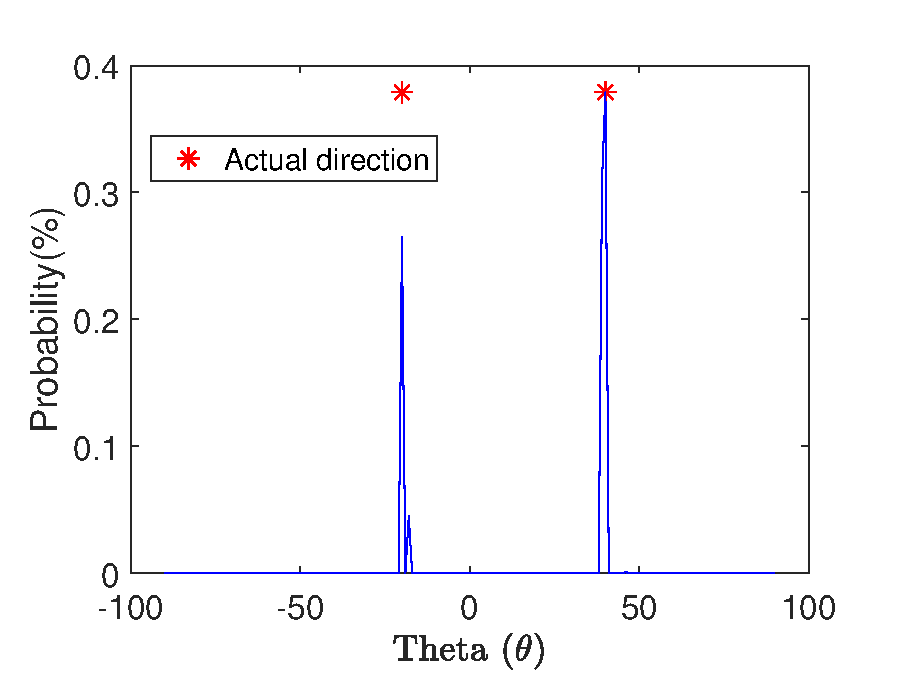
\includegraphics[width=0.7\linewidth]{N_2_30dB}
	\caption{The predicted probability with N = 2, SNR = 30 dB.}
	\label{fig:N_2_30dB}
\end{figure}     

\begin{figure}[t]
	\centering
	\includegraphics[width=0.7\linewidth]{N_3_30dB}
	\caption{The predicted probability with N = 3, SNR = 30 dB.}
	\label{fig:N_3_30dB}
\end{figure}  

\bibliography{E:/latex_biblio/huabiblio}
\bibliographystyle{IEEEtran}
\end{document}